ReversiXT ist eine Erweiterung des Brettspiels Reversi, welches in den 1880er Jahren vom Engl\"ander Lewis Waterman entwickelt wurde.
Es handelt sich um ein 2-Personen-Spiel mit einem 8x8 gro"sen Spielfeld.
Es werden je zwei Spielsteine in unterschiedlichen Farben diagonal zueinander mittig auf dem Spielfeld platziert (siehe Abbildung~\ref{fig:basicgame}).
Der blaue Spieler beginnt und darf nun auf leere Felder setzen, die ausgehend von diesem Feld in beliebiger Richtung (senkrecht, waagerecht oder diagonal) einen oder mehrere gegnerische Steine zwischen eigenen Steinen einschlie"sen.
Beim Durchf\"uhren eines Spielzuges werden die gegnerischen Spielsteine in die eigene Farbe umgef\"arbt.
Die m\"oglichen Startz\"uge wurden in der Grafik eingezeichnet.
Gewonnen hat derjenige, der zum Schluss die meisten Steine besitzt.

\vspace{1em}
\begin{minipage}{\linewidth}
	\centering
	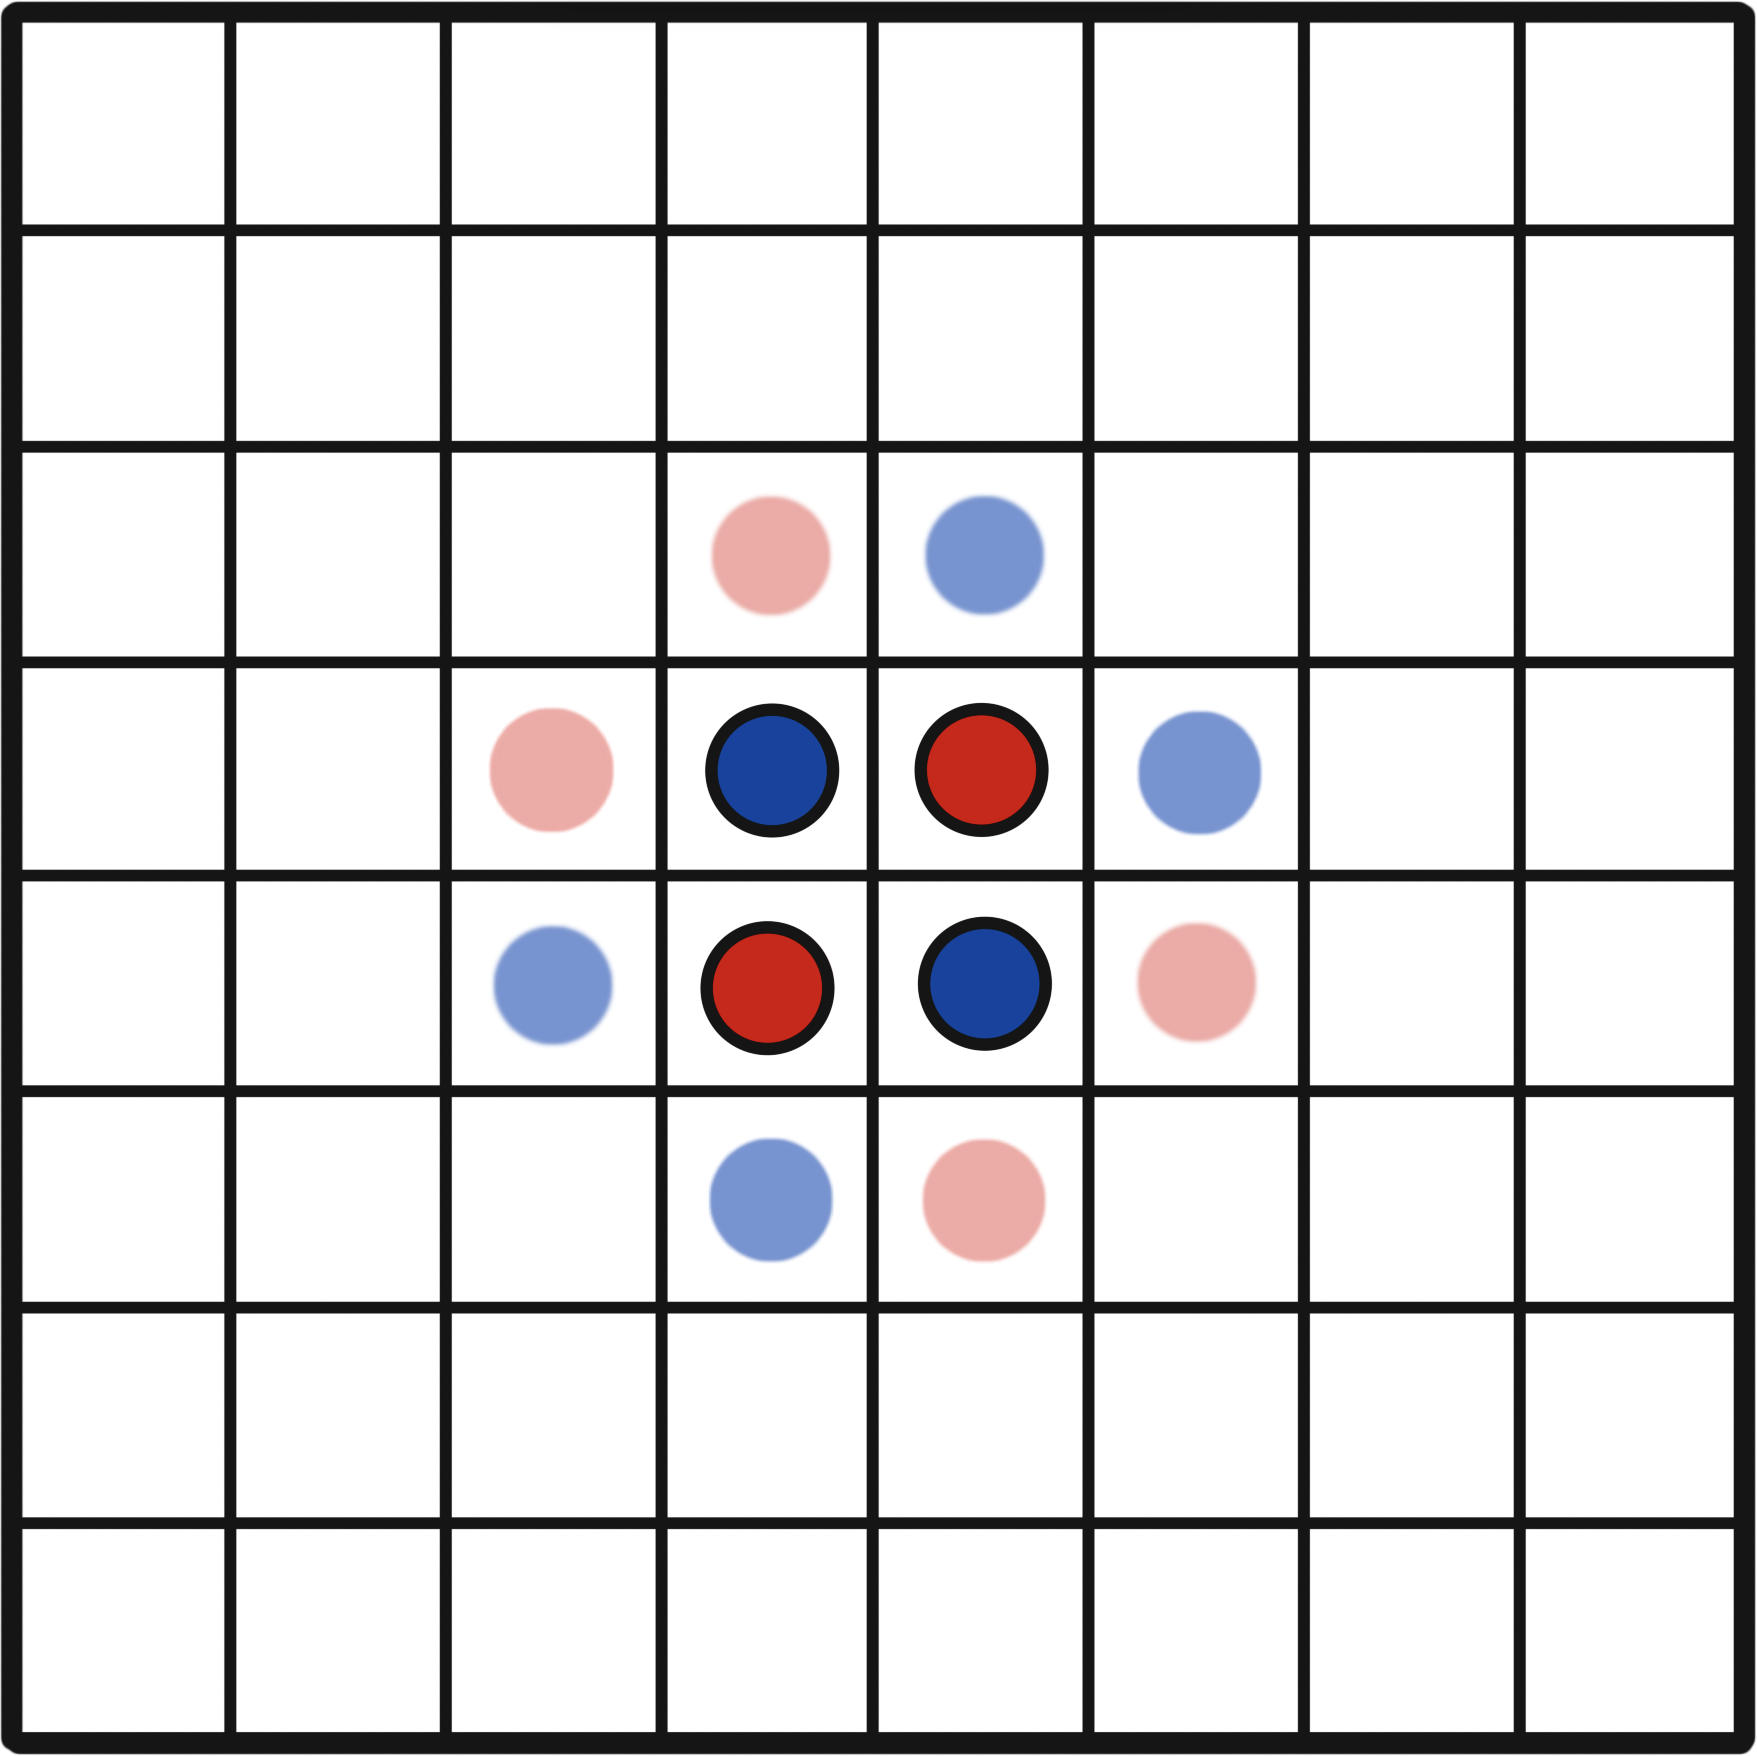
\includegraphics[width=0.5\linewidth]{pics/basicgame-start}
	\captionof{figure}[Grundspiel Start]{Grundspiel Reversi mit möglichen Startzügen}
	\label{fig:basicgame}
\end{minipage}

\subsection{Besonderheiten von ReversiXT}\label{subsec:besonderheiten-von-reversixt}
Das Spiel ReversiXT, welches als Reversi Extreme bezeichnet wird, basiert auf den gleichen Regeln wie das Grundspiel Reversi.
Es beinhaltet jedoch einige Zusatzregelungen, welche hier kurz erkl\"art werden.
Bei ReversiXT treten bis zu acht Spieler auf einem maximal 50x50 gro"sen Spielfeld gegeneinander an.
Das Spiel besteht dabei aus zwei unterschiedlichen Spielphasen.
In Phase 1 m\"ussen Spieler solange ziehen, bis kein Zug mehr m\"oglich ist.
Im Anschluss beginnt die Phase 2, die sogenannte Bombenphase.
Zudem gibt es mehrere Spezialfelder, die vorab fest definiert sind und jeweils nur einmal ausgel\"ost werden k\"onnen.
Mit einem Inversionsfeld werden die Farben aller Spieler um eins weiter verschoben.
Mit einem Choicefeld wird ein Spieler mit einem Anderen getauscht, hier ist es auch erlaubt sich selbst zu w\"ahlen.
Ein Expansionsfeld wird als Gegner gewertet und kann nach den gleichen Regeln wie andere Spieler eingenommen werden, oder mithilfe eines \"Uberschreibsteins ohne Beachtung der Spielregeln \"uberschrieben werden.
\"Uberschreibsteine k\"onnen auch genutzt werden, um einen Gegenspieler unter Beachtung der normalen Regeln zu \"uberschreiben und dabei das Spielfeld auf gewohnte Weise einzuf\"arben.
Die Anzahl von \"Uberschreibsteinen sowie Bomben ist zu Beginn des Spieles festgelegt.
Durch ein Bonusfeld darf der Spieler zwischen einem \"Uberschreibstein und einer Bombe w\"ahlen, welche dem jeweiligen Spieler gutgeschrieben wird.
Ist es nun keinem Spieler mehr m\"oglich einen legitimen Spielzug durchzuf\"uhren, beginnt die zweite Phase.
Hierbei m\"ussen abwechselnd, sofern vorhanden, alle Bomben gesetzt werden.
Hierzu wird ein Feld ausgew\"ahlt und ein Bereich mit festgelegtem Radius weggesprengt.
Dabei werden alle Felder zu L\"ochern umgewandelt.
L\"ocher sind nicht besetzbare Felder, sozusagen tote Felder.

Eine weitere Besonderheit von ReversiXT sind Transitionen.
Eine Transition kann an einem Feld liegen, an dem in einer gewissen Zugrichtung kein Weiteres mehr existiert.
Besitzt ein solches Feld nun eine Transition in einer Richtung, in die der Spieler durch einen Spielzug ziehen m\"ochte, kommt sein Stein an einer anderen festgelegten Stelle des Spielfeldes heraus.

Im Grundspiel Reversi gelten Ecken und die damit eingenommenen Kanten als sichere Felder, da es nicht mehr m\"oglich ist, diese durch einen g\"ultigen Zug umzuf\"arben.
Im Gegensatz dazu gibt es in ReversiXT aufgrund von \"Uberschreibsteinen keine sicheren Felder, da diese einfach \"uberschrieben werden k\"onnen.
Zus\"atzlich gibt es extrem viele Besonderheiten und unvorhersehbare Abh\"angigkeiten aufgrund von Transitionen und den zuvor genannten Zusatzregeln.
Aus diesen Gr\"unden ist es f\"ur einen Menschen sehr schwer bis unm\"oglich ReversiXT erfolgreich zu spielen.

\subsection{Vorstellung vom Wahlpflichtfach}\label{subsec:vorstellung-vom-wahlpflichtfach}
Die Aufgabe in diesem Fach besteht darin, einen Client mit einer k\"unstlichen Intelligenz zur bestm\"oglichen Spielzugwahl zu entwickeln, da es Computern m\"oglich ist, alle denkbaren Spielz\"uge zu ber\"ucksichtigen und diese miteinander zu vergleichen.
Wir erwarten uns von diesem Fach Einblicke in die Entwicklung von k\"unstlicher Intelligenz zu erhalten.
Zus\"atzlich ist es das erste Projekt im Studium, bei dem in einem Team an einem gemeinsamen Projekt gearbeitet wird.
Wir erhoffen uns damit wichtige Erfahrungen bez\"uglich Softwareplanung, Teamkoordination und Arbeitsverteilung zu sammeln, die f\"ur den sp\"ateren Berufseinstieg von gro"sem Nutzen sind.
Aktuell ist zudem das Thema maschinelles Lernen in aller Munde, wobei es nicht f\"ur jedes Projekt von Vorteil ist.
Mit der Entwicklung einer k\"unstlichen Intelligenz und einer Einf\"uhrung \"uber das maschinelle Lernen wollen wir die Vor- und Nachteile beider Innovationen erkennen und hautnah die Unterschiede verstehen lernen.


\bigskip
\newpage